\documentclass[turkish]{beamer}
\usepackage{beamerthemesplit}
\usepackage[latin5]{inputenc}
\usepackage{graphicx}
\usepackage{times}
\usepackage[T1]{fontenc}
\usepackage{tikz}
\usetikzlibrary{arrows}

\title{Castle Windsor}
\author{Tuna Toksoz}
\date{\today}

\begin{document}

\frame
{
	\titlepage
}

\section[Agenda]{}
\frame{\tableofcontents}
\section{Who am I?}
	\frame
	{
	  \frametitle{Who am I?}
	 	\begin{itemize}
		  \item<1-> Senior student at Bogazici University
		  \item<2-> (Passive) committer at Castle and NHibernate
		  \item<3-> Blogger at his own blog and also on devlicio.us
		  \item<4-> Has an interest in Robotics and its applications
	  \end{itemize}
	}

\section{Introduction}
	\subsection{Dependency Injection}
		\frame
		{
		  \frametitle{What is DI all about?}
		
		  \begin{itemize}
		  \item<1-> It is a pattern in Martin Fowler's book
		  \item<2-> Depends on the principle of providing dependencies from the outside
		  \item<3-> Made up of 3 components
			  \begin{itemize}
			  	\item<4->Dependent
			  	\item<5->Dependency
			  	\item<6->Dependency provider
			  \end{itemize}
		  \end{itemize}
		}
		\frame
		{
			\frametitle{Why should we use DI?}
		  \begin{itemize}
		  	\item<1->Loosely coupled components/services
		  	\item<2->Increased testability
		  	\item<3->Reduced cost of changes in later stages of development
		  	\item<4->Ability to change implementations between testing and deployment
		  \end{itemize}
		}
		\frame
		{
			\frametitle{Why should not we use DI?}
		  \begin{itemize}
		  	\item<1-> ...
		  \end{itemize}
		}
		\frame
		{
			\frametitle{Dependency Injection Methods}
		  \begin{itemize}
		  	\item<1->Constructor Injection
		  	\item<2->Property Injection
		  	\item<3->Method Injection
		  \end{itemize}
		}
		\frame
		{
			\frametitle{Dependency Injection Methods - Examples}
		  \begin{itemize}
		  	\item<1->Constructor Injection
		  		\begin{center}
						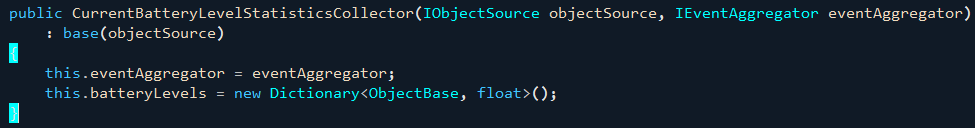
\includegraphics[scale=0.40]{images/constructorinjection.png}
					\end{center}
		  	\item<2->Property Injection
		  		\begin{center}
		  			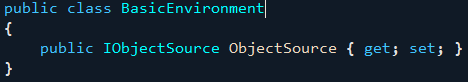
\includegraphics[scale=0.40]{images/propertyinjection.png}
		  		\end{center}
		  	\item<3->Method Injection
		  \end{itemize}
		}
	\subsection{Inversion of Control Container}
	  \frame
		{
			\frametitle{Inversion of Control Container}
			\begin{itemize}
				\item<1->A point where all components are registered and being accessed
				\item<2->A component which resolves dependencies of a requested component automatically
				\item<3->Enables us to change implementations without much trouble
			\end{itemize}
		}
\section{Castle Windsor}
	\subsection{Why Castle Windsor?}
			\frame
			{
				\frametitle{Why Castle Windsor?}
			  \begin{itemize}
			  	\item<1->A popular framework
			  	\item<2->Active development
			  	\begin{itemize}
			  	  \item<3->118 commits between October 2009 and February 2010.   
			  		\item<4->2nd version
			  	\end{itemize}
			  	\item<5->Extensibility points
			  \end{itemize}
			}
	\subsection{Configuration}
		\frame
		{
			\frametitle{Castle Windsor Configuration}
			\begin{itemize}
				\item<1->XML Configuration
				\item<2->Fluent Configuration
				\item<3->Binsor/Boo Configuration
			\end{itemize}
		}
		\frame
		{
			\frametitle{XML Configuration}
			\begin{block}{Cons}
				\begin{itemize}
					\item<1->Old school
					\item<2->Error-prone
				\end{itemize}
			\end{block}
			\begin{block}{Pros}
				\begin{itemize}
				  \item<3->Ability to change without compilation
				\end{itemize}
			\end{block}
	
			\begin{center}
				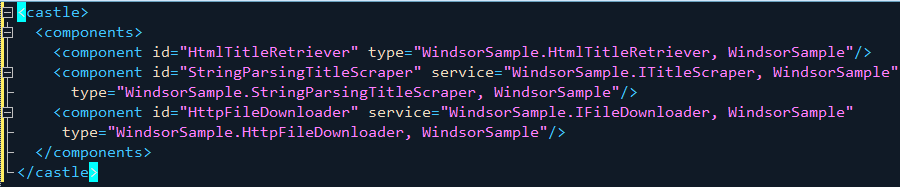
\includegraphics[scale=0.40]{images/xmlconfiguration.png}
			\end{center}
		}
	  \frame
		{
			\frametitle{Fluent/Programmatic Configuration}
			\begin{block}{Cons}
				\begin{itemize}
					\item<1->Very hard, if not impossible, to change after compilation
				\end{itemize}
			\end{block}
			\begin{block}{Pros}
				\begin{itemize}
					\item<2->Compile time checking
					\item<3->Intellisense
					\item<4->AllTypes Of
					\item<5->Convention over Configuration
				\end{itemize}
			\end{block}
		}
		\frame
		{
			\frametitle{Fluent/Programmatic Configuration - Cont'd}
			\begin{center}
				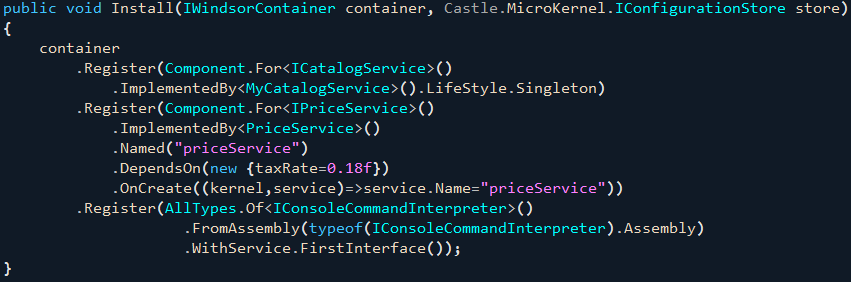
\includegraphics[scale=0.40]{images/fluentconfiguration.png}
			\end{center}
		}
		\frame
		{
			\frametitle{Boo/Binsor Configuration}
			\begin{itemize}
				\item<1->Compile/Runtime checking 
				\item<2->Intellisense (MonoDevelop)
				\item<3->Easy to change after compilation of application
				\item<4->Easier configuration with the help of Boo extensibility(macros)
			\end{itemize}
			\begin{center}
				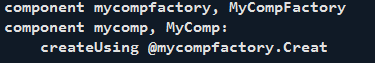
\includegraphics[scale=0.40]{images/binsorconfiguration.png}
			\end{center}
		}
	\subsection{Extensibility points}
		 \frame
			{
				\frametitle{Extensibility points}
			  \begin{itemize}
			  	\item<1->Facilities
			  	\item<2->Events
			  	\item<3->Dependency resolution control mechanisms
			  	\begin{itemize}
			  	  \item<4->Subdependency Resolver
			  		\item<5->Handler Selector
			  		\item<6->Interceptor Selector
			  	\end{itemize}
			  	\item<7->Lifestyle control mechanisms
			  	\item<8->Object initialization control mechanisms
			  \end{itemize}
			}
			\subsubsection{Facilities}
				\frame
				{
					\frametitle{Facilities}
					\begin{itemize}
						\item<1-> MK/Windsor's points of configurations
						\item<2-> A point where a group of related configuration (microkernel) tasks take place
					\end{itemize}
			  }
			  \frame
				{
					\frametitle{Available Facilities}
					\begin{itemize}
						\item<1-> Active Record Integration
						\item<2-> Automatic Transaction Management
						\item<3-> Batch Registration - Obselete
						\item<4-> Event Wiring
						\item<5-> Factory Support
						\item<6-> Nhibernate Integration
						\item<7-> Synchronize
						\item<8-> WCF Facility
					\end{itemize}
				}
			\subsubsection{Events}
				\frame
				{
					\frametitle{Eventler}
					\begin{itemize}
						\item<1-> ComponentRegistered
						\item<2-> ComponentUnregistered
						\item<3-> ComponentModelCreated
						\item<4-> ComponentCreated
						\item<5-> ComponentDestroyed
						\item<6-> DependencyResolving
						\item<7-> and several others
  				\end{itemize}
  				
				}
				\frame
				{
					\frametitle{Eventler - Code}
					\begin{center}
						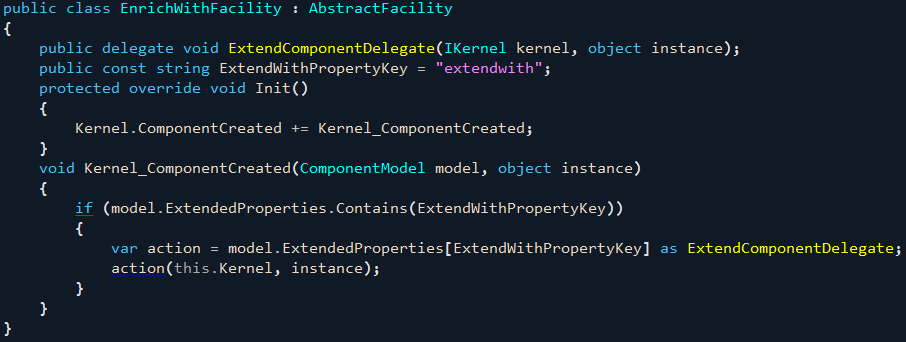
\includegraphics[scale=0.40]{images/enrichwithfacility.png}
  				\end{center}
				}
			\subsubsection{Dependency resolution control mechanisms}
				\frame
				{
					\frametitle{Dependency resolution control mechanisms}
			  	\begin{itemize}
			  	  \item<1->Subdependency Resolver
			  		\item<2->Handler Selector
			  		\item<3->Interceptor Selector
			  	\end{itemize}
			 }
			 	\frame
				{
					\frametitle{Subdependency Resolver}
			  	\begin{itemize}
			  	  \item<1->Tells \b{how} a specific dependency of a component should be resolved
			  		\item<2->We can either use an existing component or create a new one as the dependency
			  		\item<3->Does not affect previously initialized components (MEF can do it)
			  	\end{itemize}
			 }
			 	\frame
				{
					\frametitle{Subdependency Resolver - Code}
					\begin{center}
						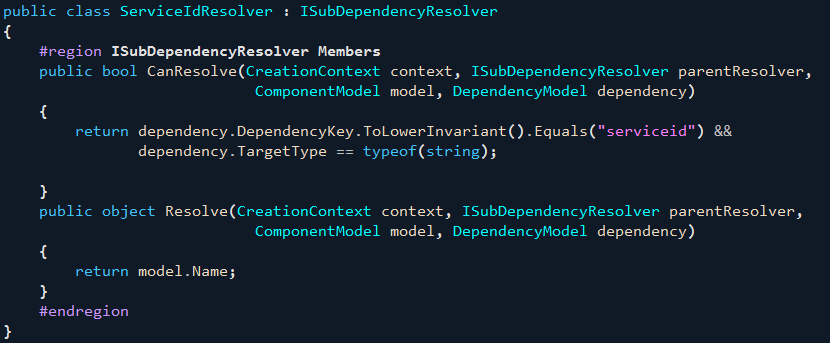
\includegraphics[scale=0.40]{images/serviceidresolver.png}
					\end{center}
			  }
			 	\frame
				{
					\frametitle{Subdependency Resolver - Code 2}
					\begin{center}
						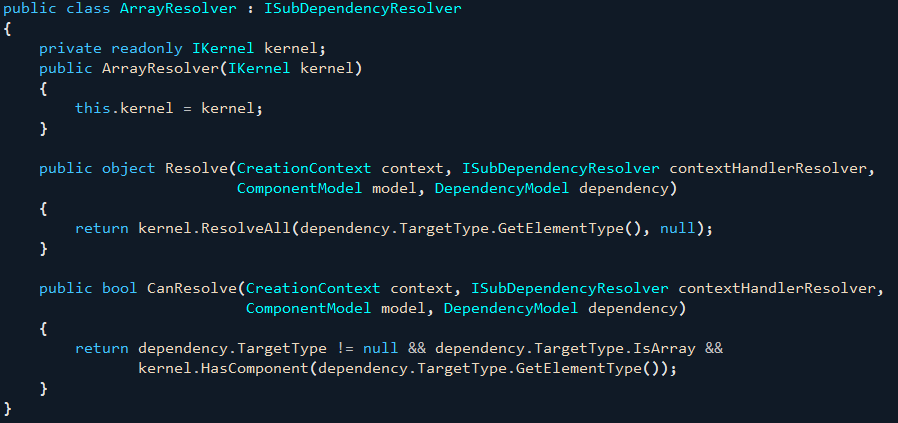
\includegraphics[scale=0.40]{images/arrayresolver.png}
					\end{center}
					\newline
					\b{Spot the potential problem}			  
				}				
				\frame
				{	
					\frametitle{Handler Selector}
			  	\begin{itemize}
			  		\item<1->Allows us to specify what to return as a result of .Resolve<T> calls depending on context 
			  		\item<2->Does not affect previously initialized components
			  	\end{itemize}
			 }
			 	\frame
				{
					\frametitle{Handler Selector - Code}
					\begin{center}
						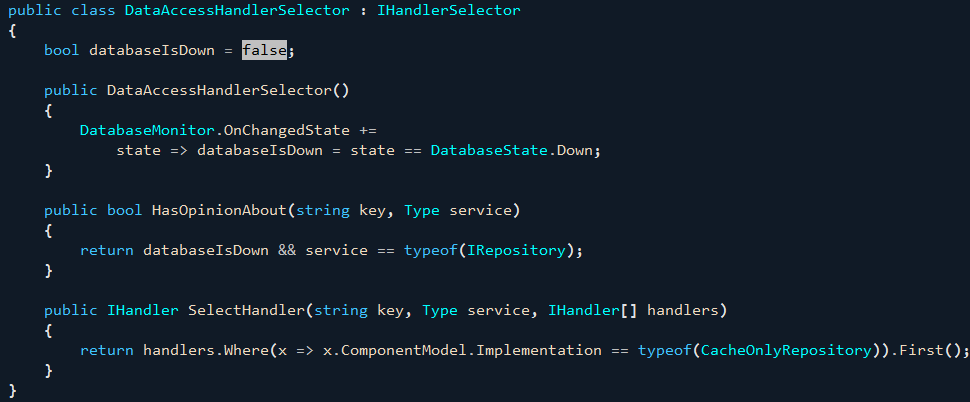
\includegraphics[scale=0.40]{images/handlerselector.png}
					\end{center}
	    	 }
	    	\frame
				{
					\frametitle{Interceptor Selector/Interceptor Model Selector/IProxyGeneration Hook}
			  	\begin{itemize}
			  	  \item<1->Allows us to change cross-cutting concerns at runtime
			  		\item<2->We can specify what interceptors should be attached
			  		\item<3->Allows us to specify what methods to intercept
			  	\end{itemize}
			 }
		\subsubsection{Lifestyle control mechanisms}
			  \frame
				{
					\frametitle{Lifestyle control mechanisms}
					Decides \b{when} to create a component
			  	\begin{itemize}
			  	  \item<1->Singleton
			  	  \item<2->PerThread
			  	  \item<3->PerWebRequest
			  	  \item<4->Transient
			  	  \item<5->Poolable
			  	  \item<6->Custom
			  	\end{itemize}
			 }
			 \frame
			{
				\frametitle{Available Lifestyles - Singleton}
				\begin{center}
						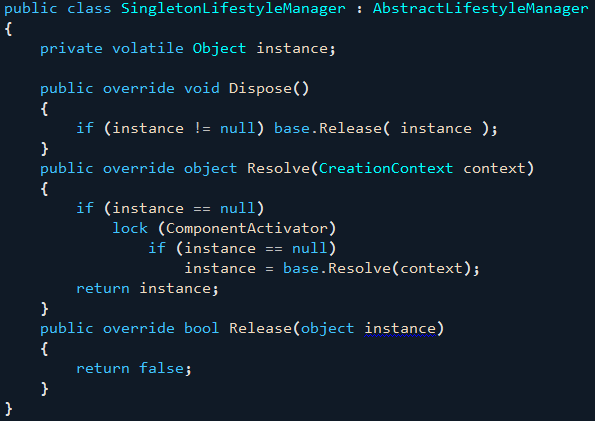
\includegraphics[scale=0.50]{images/singletonlifestylemanager.png}
				\end{center}
	    }
			\subsubsection{Component initialization control mechanisms}
			  \frame
				{
					\frametitle{Component initialization control mechanisms}
					Contains the logic related to creation of components. They are called Activators in Castle terms.
			  	\begin{itemize}
			  		\item<1->Default Activator (The place where dependency injection basically takes place)
			  		\item<2->Accessor/Factory Activator (Used by Factory Support Facility)
			  	\end{itemize}
			 }
			 	\frame
				{
					\frametitle{Component initialization control mechanisms - Accessor Activator}
					\begin{center}
							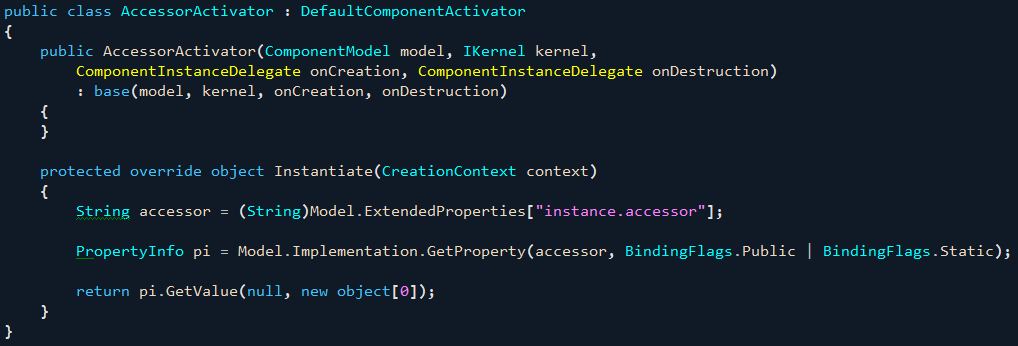
\includegraphics[scale=0.40]{images/accessoractivator.png}
					\end{center}
			  }
	\section{Conclusion}
		 \frame
		 {
		  	\frametitle{DI Advantages}
				\begin{itemize}
					\item<1->Reduced cost of change
			  	\item<2->Increased testability
			  	\item<3->Allows us to think in terms of component
			  \end{itemize}
			}
			\frame
		 {
		  	\frametitle{Windsor}
				\begin{itemize}
					\item<1->A framework that is developed as a result of needs
			  	\item<2->Easy integration with other frameworks
			  	\item<3->Active development
			  \end{itemize}
			}
			\frame
		 {
		  	\frametitle{Resources}
				\begin{itemize}
					\item<1->\href{http://castleproject.org}{http://castleproject.org}
					\item<2->\href{http://groups.google.com/group/castle-project-users/}{http://groups.google.com/group/castle-project-users/}
			  	\item<3->\href{http://ayende.com}{http://ayende.com}
			  \end{itemize}
			}
\end{document}
